\chapter{Week 5 - Challenges in the Third World}
\textit{02-10-2017 \\
Henny Romijn}

\section{What is wrong with the concept of "Third World"?}
"Third World" is an old term from the Cold War era during the 70s. A better concept for the 21st century is the global south. \\
\\
The South is a heterogeneous bunch ranging from BRICS to the Least Developed Countries (LDDs). The LDCs have a very low average income per capita.

\section{What are the historical mechanisms resulting in the unequal distribution of wealth in the global south?}
Dependency movement: chronic poverty and inequality results from the way poor countries have been historically tied into the world economy by imperialism and colonialism. Latecomers cannot easily free themselves from historical structures and institutions built for low-cost natural resource extraction and cheap labor use.

\section{How is SD seen from a South perspective?}
Many criticize the core of the western development model:
\begin{itemize}
\item The promise of modernization has delivered wealth for a few, and chronic impoverishment for many;
\item The lack of ‘Trickle down’: an economic system in which the poorest gradually benefit as a result of the increasing wealth of the richest.
\begin{figure}[ht]
\begin{center}
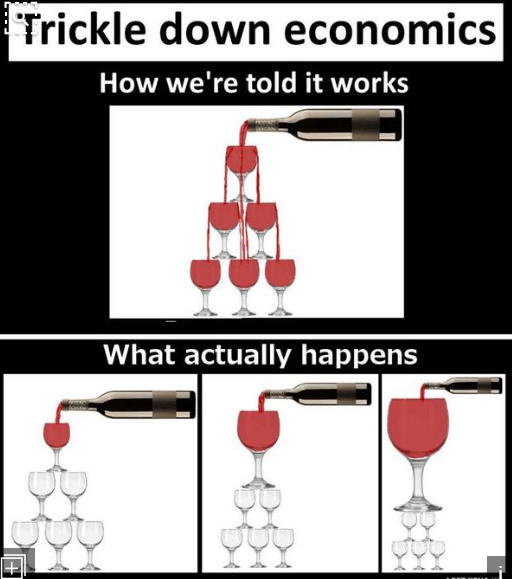
\includegraphics[scale=0.6]{Trickledown}
\end{center}
\end{figure}
\item The creation of durable exploitative capitalist relations between the world’s core and its periphery (in the sense of South).
\end{itemize}

\section{What are the six controversial South SD themes?}
\begin{enumerate}
\item Poverty: MDG effort only partly successful, hence, new 17 SDG programma started and to be achieved by 2030;
\item Food security;
\item Role of women: often excluded from policy making but can be a great force in SD;
\item Trade and SD: The WTO has its main aim of upholding the principles of free international trade and punishing trade discrimination. However, WTO is known for nontransparent decision making dominated by rich-country experts via "back-room-deals". Not surprisingly, WTO meetings have been a prime target for pro-SD activists;
\item The role of science and technology and knowledge: science and technology is often narrowed to western practices, neglecting global south knowledge and freedom;
\item Finance for SD: due to its powerful position in development finance, the World Bank is able to impose “good governance” aid financing conditions on poor countries. The World Bank emphasizes not only competent, non-corrupt government but also neoliberal policies in LDCs. These conditions are widely seen as controversial.
\end{enumerate}

\clearpage

